\documentclass{subfiles}
\begin{document}
	\par Inicialmente, foi conduzida uma pesquisa exploratória, aplicando questionários com pessoas que trabalham na área, obtendo por volta de 35 respostas, cujos resultados se encontram no [????]. Em paralelo a isso, foi realizada uma pesquisa exploratória bibliográfica em busca de softwares da área, cujos resultados estão na tabela [???]. Com estes dados em mãos, foi implementado o sistema. Por fim, foi feita uma análise quantitativa de uma pesquisa de satisfação empregada com os XX dos participantes iniciais. Resultados são descritos na seção ???.

	\par Está sendo realizada uma pesquisa de campo,

	%%%%%%%%%%%%%%%%%%%%%%%%%%%%%%%%%%%
	%%%    Tecnologias Adotadas    %%%%
	%%%%%%%%%%%%%%%%%%%%%%%%%%%%%%%%%%%
	\subsection{Tecnologias Adotadas}

		\par As seguintes tecnologias foram adotadas na construção deste projeto:

		\begin{itemize}
			\item Linguagem de Programação C, como implementada pelo compilador GCC 8.3: https://gcc.gnu.org;
			\item Linguagem de Programação C++, como implementada pelo compilador GCC 8.3: https://gcc.gnu.org/;
			\item Biblioteca multiplataforma de GUI wxWidgets, disponível em https://wxwidgets.org;
			\item Biblioteca de geração de gráficos Cairo, disponível em https://cairographics.org/;
			\item Biblioteca de manipulação de banco de dados SQLite, disponível em https://sqlite.org/.
		\end{itemize}

	%%%%%%%%%%%%%%%%%%%%%%%%%%%%%%%%%%%
	%%%    Ferramentas Adotadas    %%%%
	%%%%%%%%%%%%%%%%%%%%%%%%%%%%%%%%%%%
	\subsection{Ferramentas Adotadas}

		\par Além disso, foram utilizadas as seguintes ferramentas:

		\begin{itemize}
			\item O \textit{debugger} valgrind, disponível em: https://valgrind.org/;
			\item O editor de texto Atom, disponível em: https://atom.io/;
			\item A ferramenta de versionamento Git, disponível em: https://git-scm.com/;
			\item O site de hospedagem de projetos GitHub, disponível em: https://github.com/;
			\item O sistema Operacional Debian, disponível em: https://debian.org/;
			\item O sistema Operacional Windows, disponível em: https://microsoft.com/windows;
			\item A ferramenta UML Astah, disponível em: https://astah.net/;
			% ferramenta de pdf
		\end{itemize}
		\par As principais ferramentas adotas foram: brModelo e astah na modelagem; gcc na compilação em sistemas GNU/Linux; mingw na compilação em Windows; valgrind no debbuging; Atom na edição de texto; e \LaTeX \, na escrita do texto.

	%%%%%%%%%%%%%%%%%%%%%%%%%%%%%%%%%%%
	%%%    Modelagem do Sistema    %%%%
	%%%%%%%%%%%%%%%%%%%%%%%%%%%%%%%%%%%
	\subsection{Modelagem do Sistema}

		% A solução proposta pode ser dita como \textit{exaustiva}, no sentido de que dados tempo e memória suficientes, pode-se encontrar a melhor solução

		% É utilizada uma Decision Tree para a seleção de períodos, horários e professores no sistema.

		% \lipsum[1]

		%%%%%%%%%%%%%%%%%%%%%%%%%%%%%%%%%%%
		%%%        Casos de Uso        %%%%
		%%%%%%%%%%%%%%%%%%%%%%%%%%%%%%%%%%%
		\subsubsection{Casos de Uso}

			\par O diagrama de casos de uso, como definido por ...

			\begin{figure}[h!]
				\centering
				\fbox{
					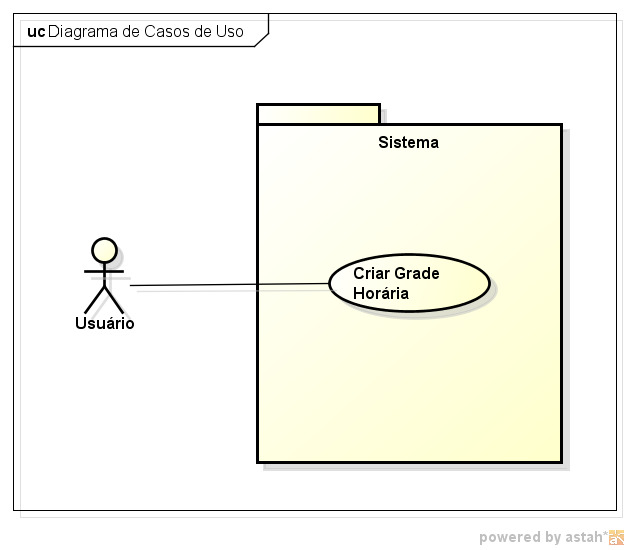
\includegraphics[width=0.5\textwidth]{CdU.jpeg}
				}
				\caption{Diagrama de Casos de Uso do Programa}
				\label{fig:cdu}
			\end{figure}

			\paragraph{ Caso de Uso 1:}

			\begin{figure}[h!]
				\centering
				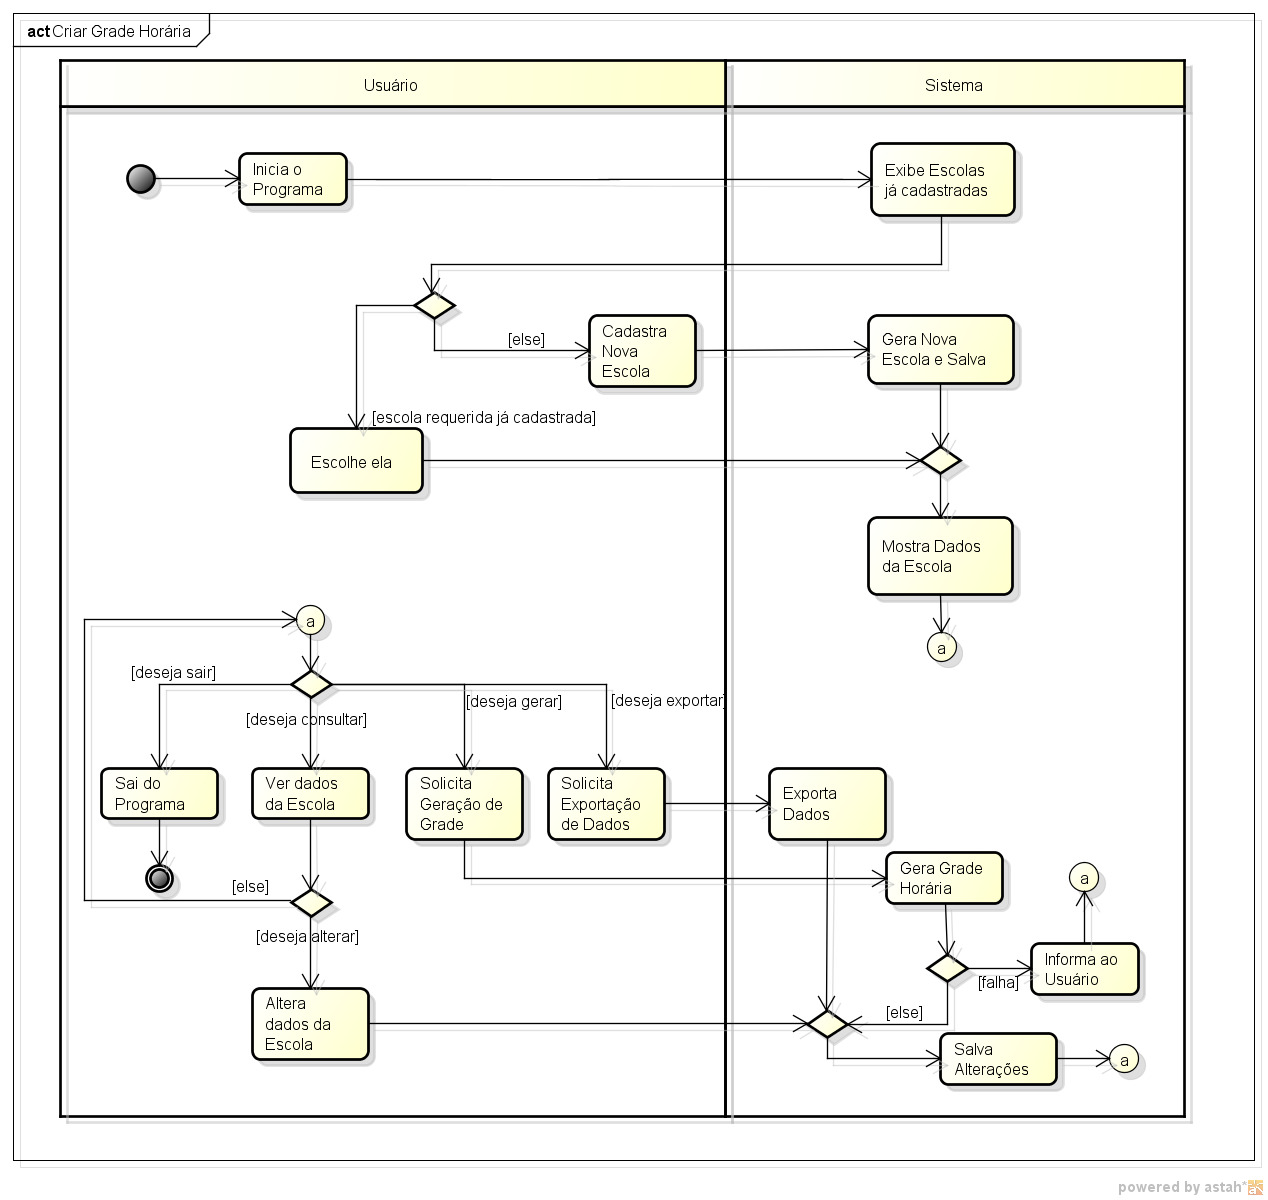
\includegraphics[width=0.7\textwidth]{Atividades.jpeg}
				\captionof{figure}{Diagrama de Atividades referente ao CdU1. Fonte: Autoria Própria}
				\label{fig:act1}
			\end{figure}

		%%%%%%%%%%%%%%%%%%%%%%%%%%%%%%%%%%%
		%%%       Banco de Dados       %%%%
		%%%%%%%%%%%%%%%%%%%%%%%%%%%%%%%%%%%
		\subsubsection{Modelagem do Banco de Dados}
			\par Todos os dados que o usuário insere no programa (exceto configurações de exibição) são armazenados em um único arquivo, denominado \textit{Database.db}. São utilizadas 35 tabelas ao total, como consta na figura \ref{fig:logico}.

			\begin{figure}[h	]
				\centering
				\fbox{
				\includegraphics[width=\textwidth]{Lógico.png}
				}
				\caption{Diagrama Lógico do Programa. Fonte: Autoria Própria}
				\label{fig:logico}
			\end{figure}

			\lipsum[1]

		% %%%%%%%%%%%%%%%%%%%%%%%%%%%%%%%%%%%
		% %%%          Algoritmos        %%%%
		% %%%%%%%%%%%%%%%%%%%%%%%%%%%%%%%%%%%
		% \subsubsection{Algoritmos}
		%
		% 		% se basear em \cite{Pillay}
		%
		% 	\textbf{Orientações Gerais}
		%
		% 	\par Sequential method of Saturation Degree (um dos mais robustos segundo Carter, Laporte e Lee 1995. Ler o artigo!).
		% 	Lewis 2015 também vê resultados mais favoráveis no Saturation
		%
		% 	\par Ler sobre 1-opt e 2-opt (Carter, Laporte e Chinnek)
		%
		% 	\par Usar alguma aleatoridade depois do primeiro cronograma para dar mais opções para o usuário

\end{document}
